\documentclass[3p,times,procedia]{elsarticle}
\flushbottom

\usepackage{ecrc}
\usepackage[bookmarks=false]{hyperref}
\hypersetup{colorlinks,linkcolor=blue,citecolor=blue,urlcolor=blue}
\usepackage{amssymb}
\usepackage{booktabs}
\usepackage{graphicx}

\volume{00}
\firstpage{1}
\journalname{Procedia Computer Science}
\runauth{Sanap et al.}
\jid{procs}
\biboptions{numbers,sort&compress}

\begin{document}
\begin{frontmatter}

\dochead{International Conference on Machine Learning and Data Engineering}

\title{Beyond Same-Corpus Accuracy: A Cross-Source Study of Hindi Audio Deepfake Detection}

\author[kkw]{Prathmesh Pravin Sanap}
\author[kkw]{Shivam Vinod Shewale}
\author[kkw]{Yash Vinayak Jadhav}
\author[kkw]{Snehal Sandeep Sanap}

\address[kkw]{Department of Computer Engineering, K. K. Wagh Institute of Engineering Education and Research, Nashik 422003, Maharashtra, India}

\begin{abstract}
Evaluation within a single corpus can give an unrealistic view of an audio
deepfake detector. This work measures that gap for Hindi speech using a
leakage-checked, transcript-grouped protocol. We formed 3,000 bona
fide--spoof pairs from SEA-Spoof, trained EfficientNet-B0 independently with
three seeds, and kept every pair inside one data partition. Each frozen model
was then evaluated on unseen genuine speech from Kathbath and Common Voice
and unseen synthetic speech from IndicSynth. The internal SEA-Spoof tests
gave accuracies from 99.50\% to 100\%. Across the external tests, balanced
accuracy was $89.07\%\pm1.15\%$, ROC-AUC was $0.9501\pm0.0205$, and EER was
$10.98\%\pm3.69\%$. The aggregate result concealed a concentrated failure:
the mean correct-classification rate for genuine Kathbath clips was 39.44\%,
whereas the three remaining sources each exceeded 98.6\%. Earlier
source-rotation checks also produced EERs from 3.74\% to 40.46\%, indicating
strong sensitivity to corpus composition. Thus, controlling transcript
content prevents text overlap from leaking across partitions, but does not
remove channel and corpus effects. Hindi deepfake studies should therefore
report both leakage audits and results separated by unseen source.
\end{abstract}

\begin{keyword}
audio deepfake detection \sep Hindi speech \sep cross-source evaluation
\sep transcript pairing \sep EfficientNet \sep source bias
\end{keyword}

\end{frontmatter}
\vspace*{-6pt}

\section{Introduction}
Modern text-to-speech and voice-conversion systems can create convincing
synthetic speech. This creates risks for voice authentication, media
verification, and digital forensics. A detector must therefore do more than
separate examples in one benchmark. It should also work when speakers,
recording devices, codecs, and synthesis systems change.

This requirement is difficult to measure. Real and fake clips often come
from different datasets. A model can then learn which dataset produced a
clip instead of learning general signs of synthesis. Random train--test
splits make this problem worse because every source appears in both parts of
the experiment. Prior work reports large losses when audio deepfake
detectors are moved to unseen data \cite{muller2022generalize,muller2024harder}.
Recent reviews likewise identify feature choice, dataset coverage, and
cross-domain evaluation as central concerns for practical detectors
\cite{salih2025review,zhang2025survey}.

We investigate this problem for Hindi. Our first pooled experiment achieved
perfect test scores, but source-held-out results varied widely. Signal and
embedding checks suggested that recording and silence patterns were acting
as shortcuts. We then built a larger experiment using transcript-paired
SEA-Spoof data \cite{wu2025seaspoof}. Each selected transcript had one real
and one fake clip, and all clips with the same transcript were kept in one
partition.

The paper contributes a leakage-checked Hindi deepfake protocol, a
three-seed external evaluation, and a source-level analysis that identifies
Kathbath as the main failure case. We do not claim that transcript pairing
is better than ordinary sampling because that claim requires a count-matched
non-paired control.

\section{Related work}
Survey and comparative studies cover a broad range of spectral
representations and neural classifiers
\cite{salih2025review,verma2025comparative,zhang2025survey}. Strong results
inside a benchmark do not, however, establish performance on a new corpus.
Our study therefore emphasizes source-held-out Hindi testing rather than a
new feature-fusion architecture.

M{\"u}ller et al. \cite{muller2022generalize} compared detection systems under
a common setup and showed that performance can fall sharply outside known
benchmarks. Their later analysis found that cross-domain failure is driven
mainly by differences between domains, not simply by one domain containing
harder fakes \cite{muller2024harder}. Kawa et al. \cite{kawa2022attack}
used disjoint attacks to study generalization. Pascu et al.
\cite{pascu2024calibrated} showed that frozen self-supervised speech
representations with a small classifier can also generalize well.

Hindi has fewer deepfake benchmarks than English. SEA-Spoof provides paired
real and spoof speech for Hindi and other Asian languages
\cite{wu2025seaspoof}. Kathbath contains labelled speech across 12 Indian
languages \cite{javed2022indicsuperb}. IndicSynth provides synthetic speech
for low-resource Indian languages \cite{sharma2025indicsynth}. Common Voice
is a crowdsourced multilingual speech corpus \cite{ardila2020commonvoice}.

\section{Data and protocol}
Table \ref{tab:data} lists the datasets used in the final experiment.
SEA-Spoof is the only training source. The other datasets are used only for
external evaluation.

\begin{table}[h]
\caption{Datasets used in the final experiment.}
\label{tab:data}
\begin{tabular*}{\hsize}{@{\extracolsep{\fill}}llll@{}}
\toprule
Dataset & Label & Role & Count \\
\colrule
SEA-Spoof Hindi & Real+fake & Train/val/test & 6,000 total \\
Kathbath Hindi & Real & External test & 100 \\
Common Voice male & Real & External test & 100 \\
Common Voice female & Real & External test & 100 \\
IndicSynth Hindi & Fake & External test & 100 \\
\botrule
\end{tabular*}
\end{table}

We selected 3,000 Hindi transcripts from the SEA-Spoof training split. For
each transcript, we kept one bona fide clip and one spoof clip. The final
corpus contained 6,000 clips. The audit found 3,000 complete transcript
groups, no missing transcripts, no duplicated paths, and no transcript that
crossed partitions. For each run, transcript groups were shuffled using the
training seed and split 80/10/10. This gave 4,800 training, 600 validation,
and 600 same-corpus test clips, with equal class counts.

Each trained model was evaluated on three deterministic external manifests.
Each manifest contained 100 clips from Kathbath, Common Voice male, Common
Voice female, and IndicSynth. A manifest therefore had 300 real and 100 fake
clips. Because the classes were not balanced, we emphasize balanced
accuracy, EER, and ROC-AUC. The sampling seeds were 42, 1337, and 2026.

Figure \ref{fig:paired} is an output of our feature-inspection script. It was
drawn directly from the saved NumPy (\texttt{.npy}) arrays used as model
inputs; it is not an illustrative or externally generated spectrogram. The
real and spoof clips contain the same transcript. The signed difference map
is included only to make differences between the two stored feature arrays
visible. It does not explain the model's decision.

\begin{figure}[h]
\centering
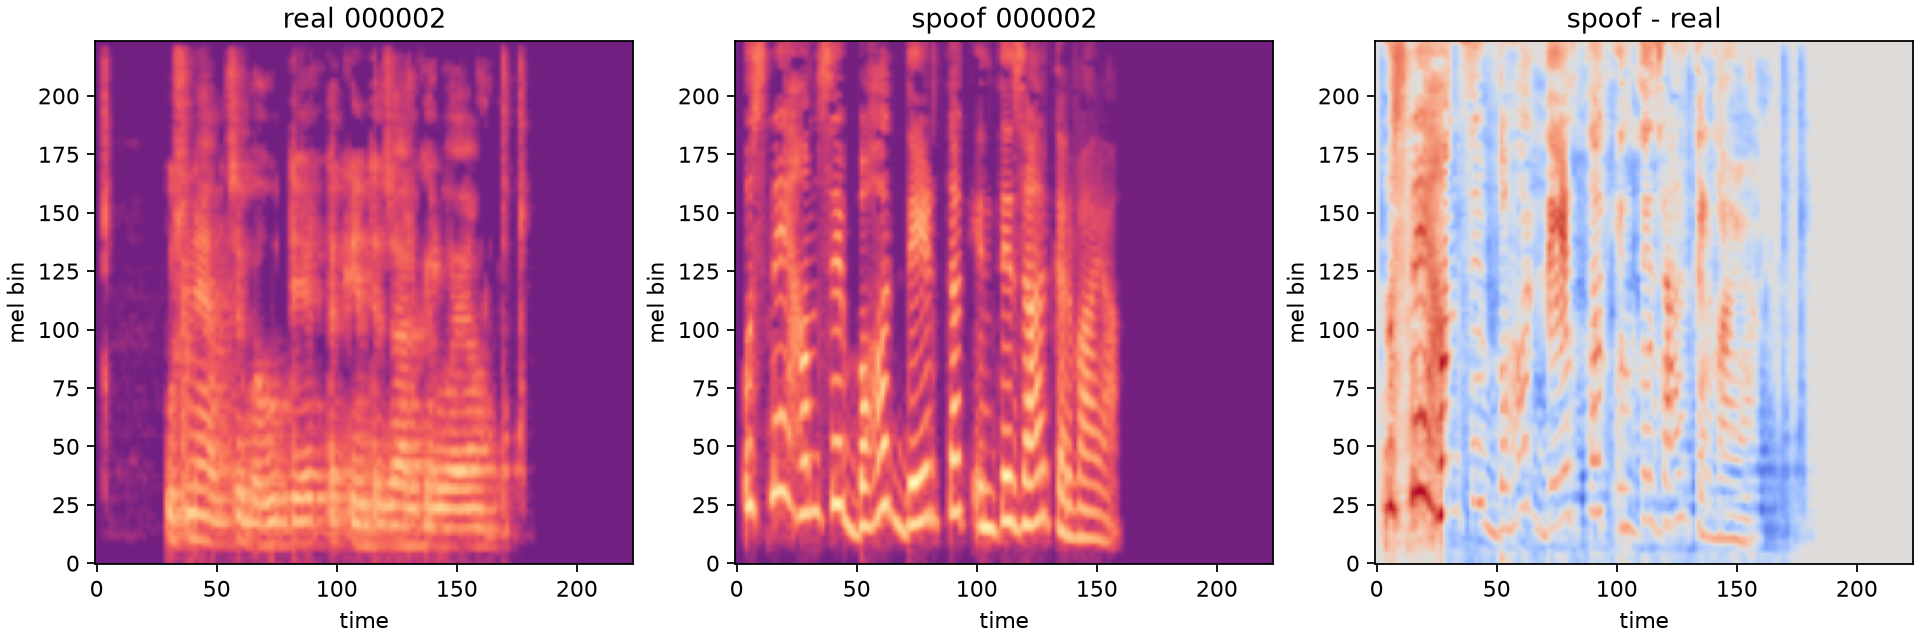
\includegraphics[width=\hsize]{figures/candidate_pairs/pair_000002.png}
\caption{Project-generated feature visualization for transcript-matched
SEA-Spoof pair 000002: bona fide (left), spoof (centre), and the element-wise
signed difference, spoof minus bona fide (right). The plot was produced
directly from the two saved $224\times224$ log-mel NumPy arrays. Thus, the
displayed time and mel-bin ticks denote resized feature-map coordinates,
not seconds and physical frequency values.}
\label{fig:paired}
\end{figure}

\section{Experimental setup}
Table \ref{tab:setup} gives the complete configuration used in all three
reported training runs. Unless a seed is stated, every setting was held
fixed. The same audio and feature pipeline was applied to SEA-Spoof and to
all external datasets. Figure \ref{fig:pipeline} summarizes the complete
training and evaluation flow.

\begin{figure}[h]
\centering
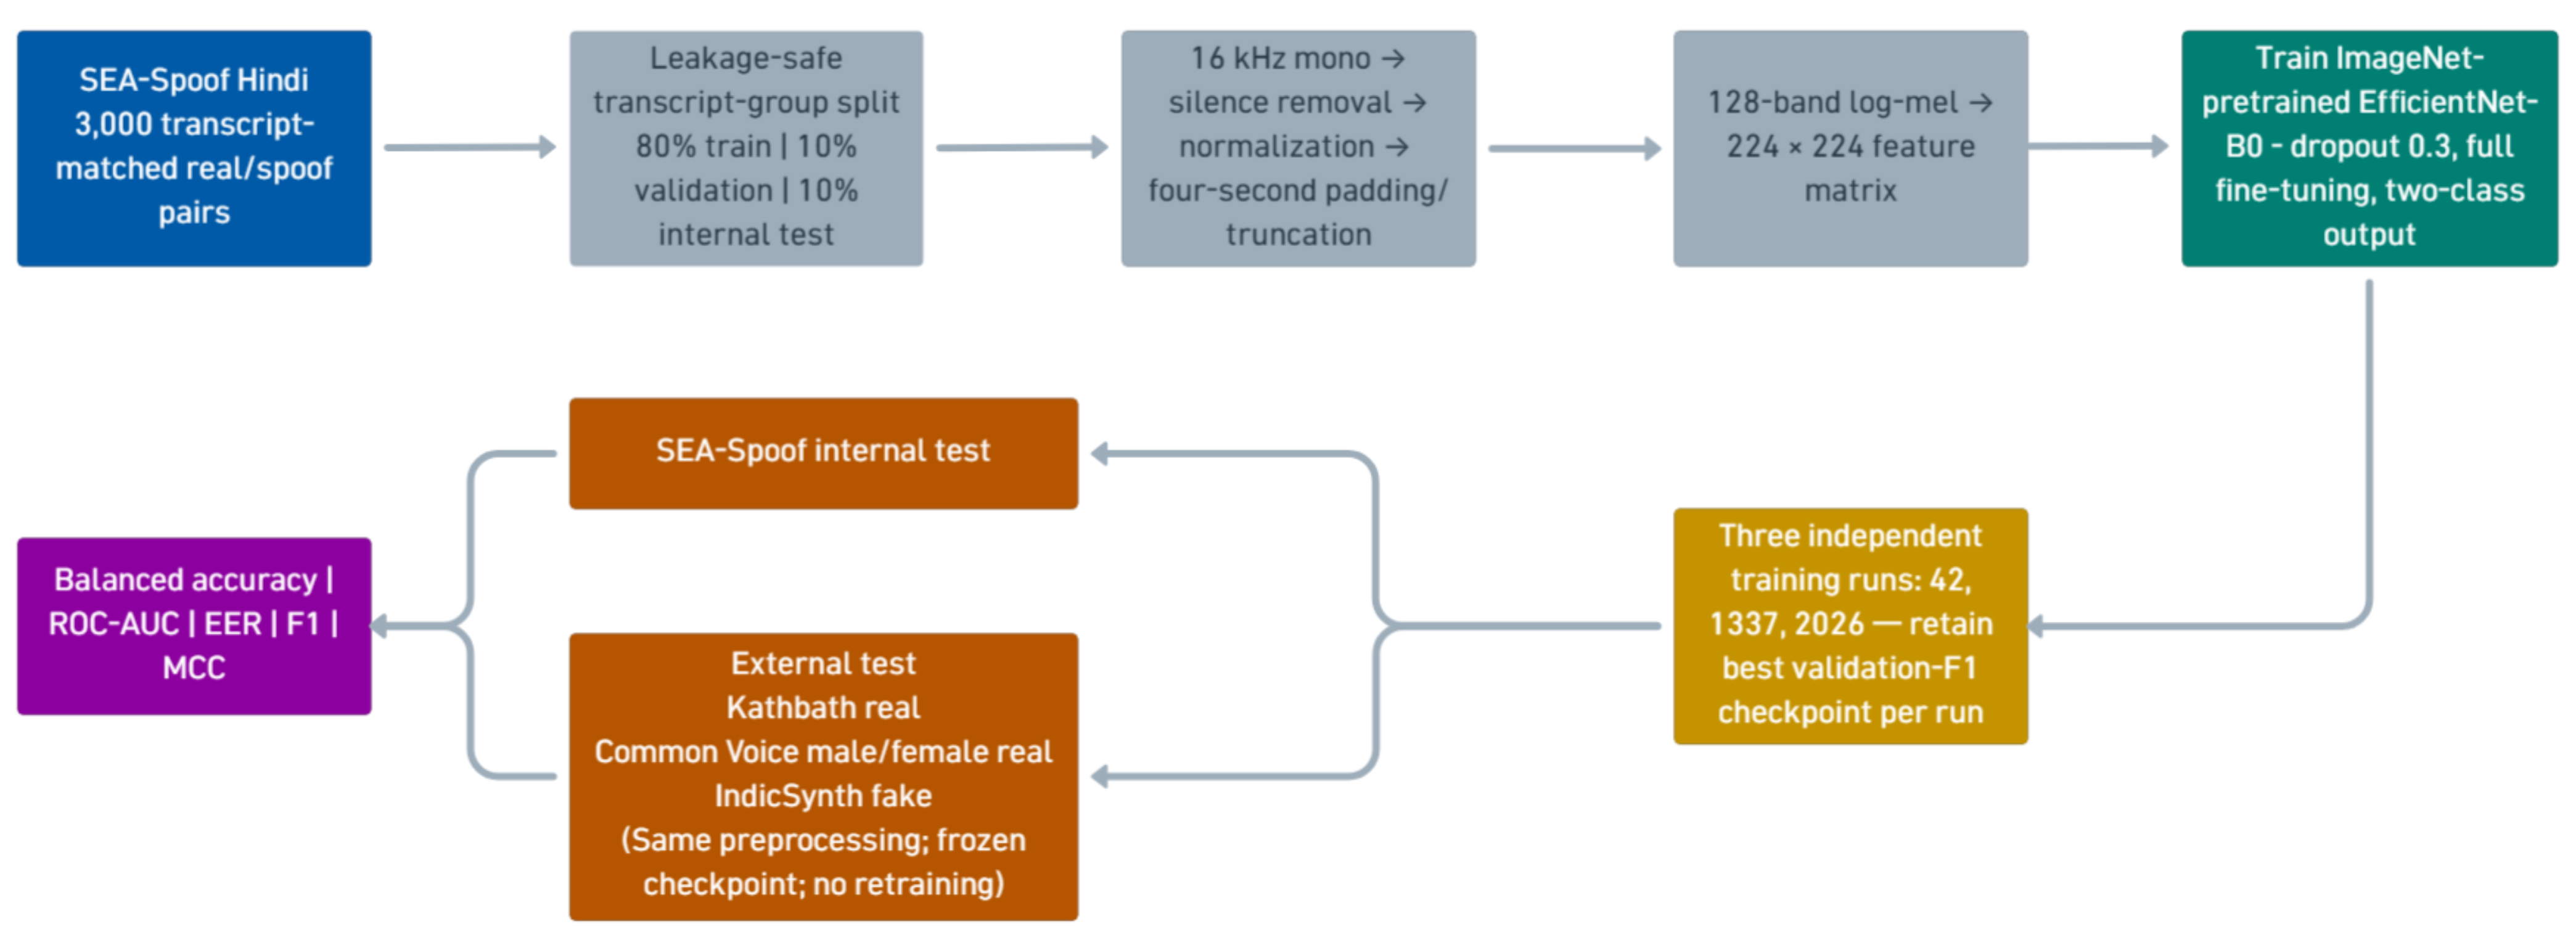
\includegraphics[width=\hsize]{figures/experimental_pipeline.png}
\caption{Leakage-safe training and evaluation pipeline. Three independently
trained models were tested internally and on unseen sources. External audio
used the same preprocessing and each checkpoint remained frozen.}
\label{fig:pipeline}
\end{figure}

\begin{table}[h]
\caption{Fixed experimental configuration.}
\label{tab:setup}
\small
\begin{tabular*}{\hsize}{@{\extracolsep{\fill}}lp{0.66\hsize}@{}}
\toprule
Component & Setting \\
\colrule
Training data & 3,000 Hindi SEA-Spoof transcripts; one bona fide and one spoof clip per transcript (6,000 clips) \\
Split & Transcript-grouped 80/10/10; 4,800 train, 600 validation, 600 same-corpus test; balanced labels \\
Audio & Mono, 16~kHz, silence removal at 30~dB, peak normalization, 4~s zero-pad/truncate \\
Features & Log-mel power spectrogram; 128 mel bands; FFT/window 1,024; hop 512; 0--8~kHz; resize to $224\times224$ \\
Model & ImageNet-pretrained EfficientNet-B0; one input channel; two outputs; dropout 0.3; full backbone fine-tuning; no BiLSTM \\
Training & Cross-entropy, AdamW, learning rate $3\times10^{-4}$, weight decay $10^{-5}$, batch 32, cosine schedule \\
Stopping & Maximum 50 epochs; best validation-F1 checkpoint; patience 7; minimum improvement $10^{-4}$ \\
Numerics & Mixed precision on CUDA; gradient norm clipped at 5.0; four data-loader workers \\
Training seeds & 42, 1337, 2026; each controls grouped split, initialization, and batch order \\
External test & Kathbath real, Common Voice male real, Common Voice female real, IndicSynth fake; 100 clips/source/manifest \\
Evaluation repeats & Sampling seeds 42, 1337, 2026 for each trained model; frozen checkpoint and no retraining \\
Decision/reporting & Threshold 0.5; balanced accuracy, F1, MCC, ROC-AUC and EER; mean and sample SD across training seeds \\
\botrule
\end{tabular*}
\end{table}

\subsection{Preprocessing and representation}
Every clip was converted to mono at 16~kHz. Silence was removed with a
30~dB threshold. The waveform was peak-normalized and padded or truncated
to four seconds. We computed a log-mel spectrogram with 128 mel bands, a
1,024-sample FFT and window, a 512-sample hop, and a frequency range of
0--8~kHz. Each feature map was resized to $224\times224$.

\subsection{Model and optimization}
The classifier was an ImageNet-pretrained EfficientNet-B0
\cite{tan2019efficientnet}, adapted for one input channel and two output
classes. The reported models did not use BiLSTM. We fine-tuned the backbone
with AdamW, learning rate $3\times10^{-4}$, weight decay $10^{-5}$, batch
size 32, cosine scheduling, mixed precision, and gradient clipping at 5.0.
Training was limited to 50 epochs and stopped after seven epochs without an
improvement in validation F1. We evaluated the best validation-F1 checkpoint.

\subsection{Runs and evaluation conditions}
We trained models with seeds 42, 1337, and 2026. A seed controlled the
transcript split, initial weights, and batch order. We report accuracy,
balanced accuracy, F1, Matthews correlation coefficient (MCC), ROC-AUC, and
EER. For each model, we first averaged the three external manifest results.
We then calculated the mean and sample standard deviation across the three
trained models. The three evaluation-sampling seeds do not represent extra
model-training runs. They change only which external clips are sampled. No
external clip was used to update model weights or select a checkpoint.

The completed condition is transcript-paired SEA-Spoof training followed by
same-corpus and cross-source evaluation. A count-matched model trained
without transcript pairing, alternative architectures, and preprocessing
ablations were not completed and are not presented as experimental results.

\section{Pilot source-shift analysis}
Before the final experiment, four models were trained on different pairs of
real and fake sources and tested on complementary sources. Table
\ref{tab:pilot} shows that the result depended strongly on source
composition. These are single-run pilot results and are used only as
motivation.

\begin{table}[h]
\caption{Pilot source-held-out experiments.}
\label{tab:pilot}
\begin{tabular*}{\hsize}{@{\extracolsep{\fill}}llrr@{}}
\toprule
Training real & Training fake & ROC-AUC & EER \\
\colrule
Kathbath & IndicSynth & 0.9939 & 0.0374 \\
Common Voice & IndicSynth & 0.8165 & 0.2325 \\
Common Voice & SEA-Spoof & 0.8761 & 0.2160 \\
Kathbath & SEA-Spoof & 0.6273 & 0.4046 \\
\botrule
\end{tabular*}
\end{table}

Signal checks found large source differences in silence and trailing
padding. In the worst rotation, embedding separation for source identity
was almost as strong as separation for the class label. These checks do not
prove causation, but they explain why a source-resolved evaluation was
needed.

\section{Results}
On their respective held-out SEA-Spoof partitions, the three runs produced
accuracies between 0.9950 and 1.0000. These internal scores show that the
grouped task was learned after removing transcript overlap; they provide no
evidence by themselves about transfer to another corpus.

Table \ref{tab:main} reports the external result for each trained model. Each
seed row is the average of three external manifests. The final row shows the
mean and standard deviation across independently trained models.

\begin{table}[h]
\caption{Primary cross-source results across model-training seeds.}
\label{tab:main}
\begin{tabular*}{\hsize}{@{\extracolsep{\fill}}lrrr@{}}
\toprule
Seed & Balanced accuracy & ROC-AUC & EER \\
\colrule
42 & .9039 & .9625 & .0922 \\
1337 & .8828 & .9615 & .0850 \\
2026 & .8856 & .9264 & .1522 \\
\colrule
Mean & .8907 & .9501 & .1098 \\
SD & .0115 & .0205 & .0369 \\
\botrule
\end{tabular*}
\end{table}

Across the same runs, accuracy was $.8422\pm.0193$, F1 was
$.7586\pm.0217$, and MCC was $.6914\pm.0264$.

Same-corpus EER was near zero, while cross-source EER increased to 10.98\%
on average. Seed 2026 was weaker than the other models, showing why a single
training run can be misleading.

Table \ref{tab:source} shows that the loss was not spread evenly across
datasets. The models were almost perfect on Common Voice and unseen
IndicSynth fake speech. Mean Kathbath accuracy was only 39.44\%.

\begin{table}[h]
\caption{Accuracy by external source.}
\label{tab:source}
\begin{tabular*}{\hsize}{@{\extracolsep{\fill}}llrr@{}}
\toprule
Source & Label & Mean acc. & Range \\
\colrule
Kathbath & Real & 0.3944 & 0.28--0.53 \\
Common Voice male & Real & 1.0000 & 1.00--1.00 \\
Common Voice female & Real & 0.9867 & 0.97--0.99 \\
IndicSynth & Fake & 0.9878 & 0.95--1.00 \\
\botrule
\end{tabular*}
\end{table}

Most aggregate errors therefore came from real Kathbath clips being labelled
as fake. The unseen fake generator was not the main problem. This is
consistent with the earlier observation that recording and silence
properties can become shortcuts. High ROC-AUC alongside lower
fixed-threshold F1 also suggests a calibration shift.

\section{Discussion}
The experiment gives two clear results. First, same-corpus performance is an
optimistic upper bound. A model can be perfect on held-out examples from one
source and still fail on a new genuine-speech corpus. Second, errors must be
reported separately by source. An aggregate score alone would hide the
Kathbath failure.

Transcript pairing removes one shortcut: spoken text cannot occur only in
one class. It does not remove microphones, codecs, speakers, silence
patterns, or generator artifacts. Content control creates a cleaner
experiment, but it is not a complete solution to domain shift. This study
does not measure the causal gain from pairing. A fair comparison needs an
equally sized non-paired training set with the architecture, optimization,
and external manifests held fixed.

\section{Limitations and ethical considerations}
The study covers Hindi only. Speaker IDs were not preserved, so
speaker-disjoint splits could not be verified. External manifests contain
100 clips per source and overlap across sample seeds. We used three training
seeds and one model family. A count-matched non-paired control and
normalization ablation were not completed. We did not compute minimum tandem
detection cost because there was no compatible automatic speaker
verification system. Kathbath performance is too low for real-world use.

A detector output is not proof that a person acted deceptively. False
positives can wrongly label genuine speech as fake, as the Kathbath result
shows. The model should not be the only decision maker in legal, financial,
or identity-verification settings. Dataset licenses and consent conditions
must be followed, and restricted audio should not be redistributed.

\section{Conclusion}
Three transcript-paired Hindi deepfake detectors were almost perfect on
held-out SEA-Spoof data but reached 10.98\% $\pm$ 3.69\% EER on external
sources. ROC-AUC remained 0.9501 $\pm$ 0.0205. The loss was concentrated on
Kathbath genuine speech, while Common Voice and IndicSynth accuracy stayed
above 98.6\%. Same-corpus accuracy can therefore hide a large source-specific
weakness. Future work should add a count-matched non-paired control, test
silence and loudness normalization, retain speaker IDs, and compare
EfficientNet-B0 with a speech-specific baseline.

\section*{Acknowledgements}
The authors thank Prof. S. S. Bhandare for her guidance and support.

\bibliographystyle{elsarticle-harv}
\bibliography{ICMLDE_references}

\end{document}
